\begin{enumerate}
	\item L'administrateur se connecte au site avec ses identifiants. 
	\item Un nouveau bouton de navigation apparait dans la barre de navigation. 
	\item L'administrateur clique sur le bouton \textit{Admin}
	\item Il sélectionne \textit{Nouvelle Session} dans le menu déroulant. 
	\item L'administrateur atterrit sur la page d'ajout de sessions. 
	\item Il remplit le formulaire avec les bonnes informations.
	\item Il clique sur \textit{Add}
\end{enumerate}

\vspace{\baselineskip}
\begin{figure}[h]
	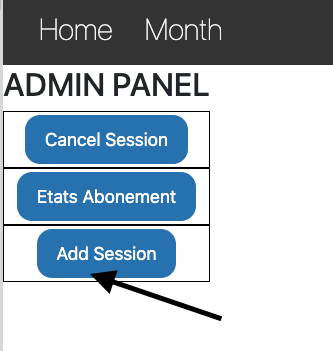
\includegraphics[width=0.4\textwidth,center]{Figures/us10-1}
	\caption{Panel de navigation de l'administrateur}
\end{figure}

\vspace{\baselineskip}
\begin{figure}[h]
	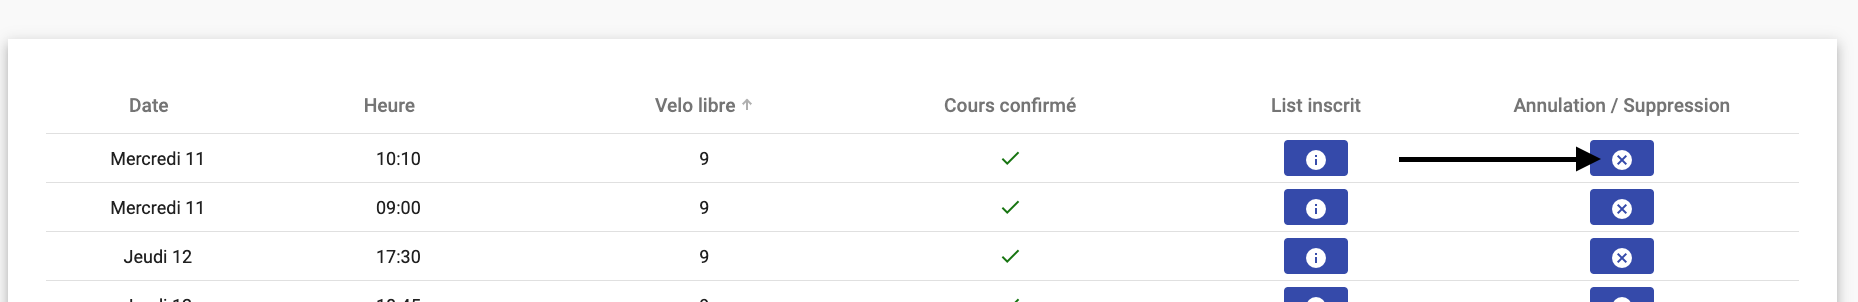
\includegraphics[width=0.6\textwidth,center]{Figures/us10-2}
	\caption{Formulaire d'ajout d'une session}
\end{figure}

\newpage
\subsubsection{Gestion des erreurs}
	\begin{itemize}
		\item Tous les champs doivent être remplis. Si ce n'est pas le cas, il sera impossible d'envoyer le formulaire et l'administrateur aura une erreur affichée.
	\end{itemize}

\newpage
\subsubsection{Diagramme de séquence}
	\begin{figure}[h]
		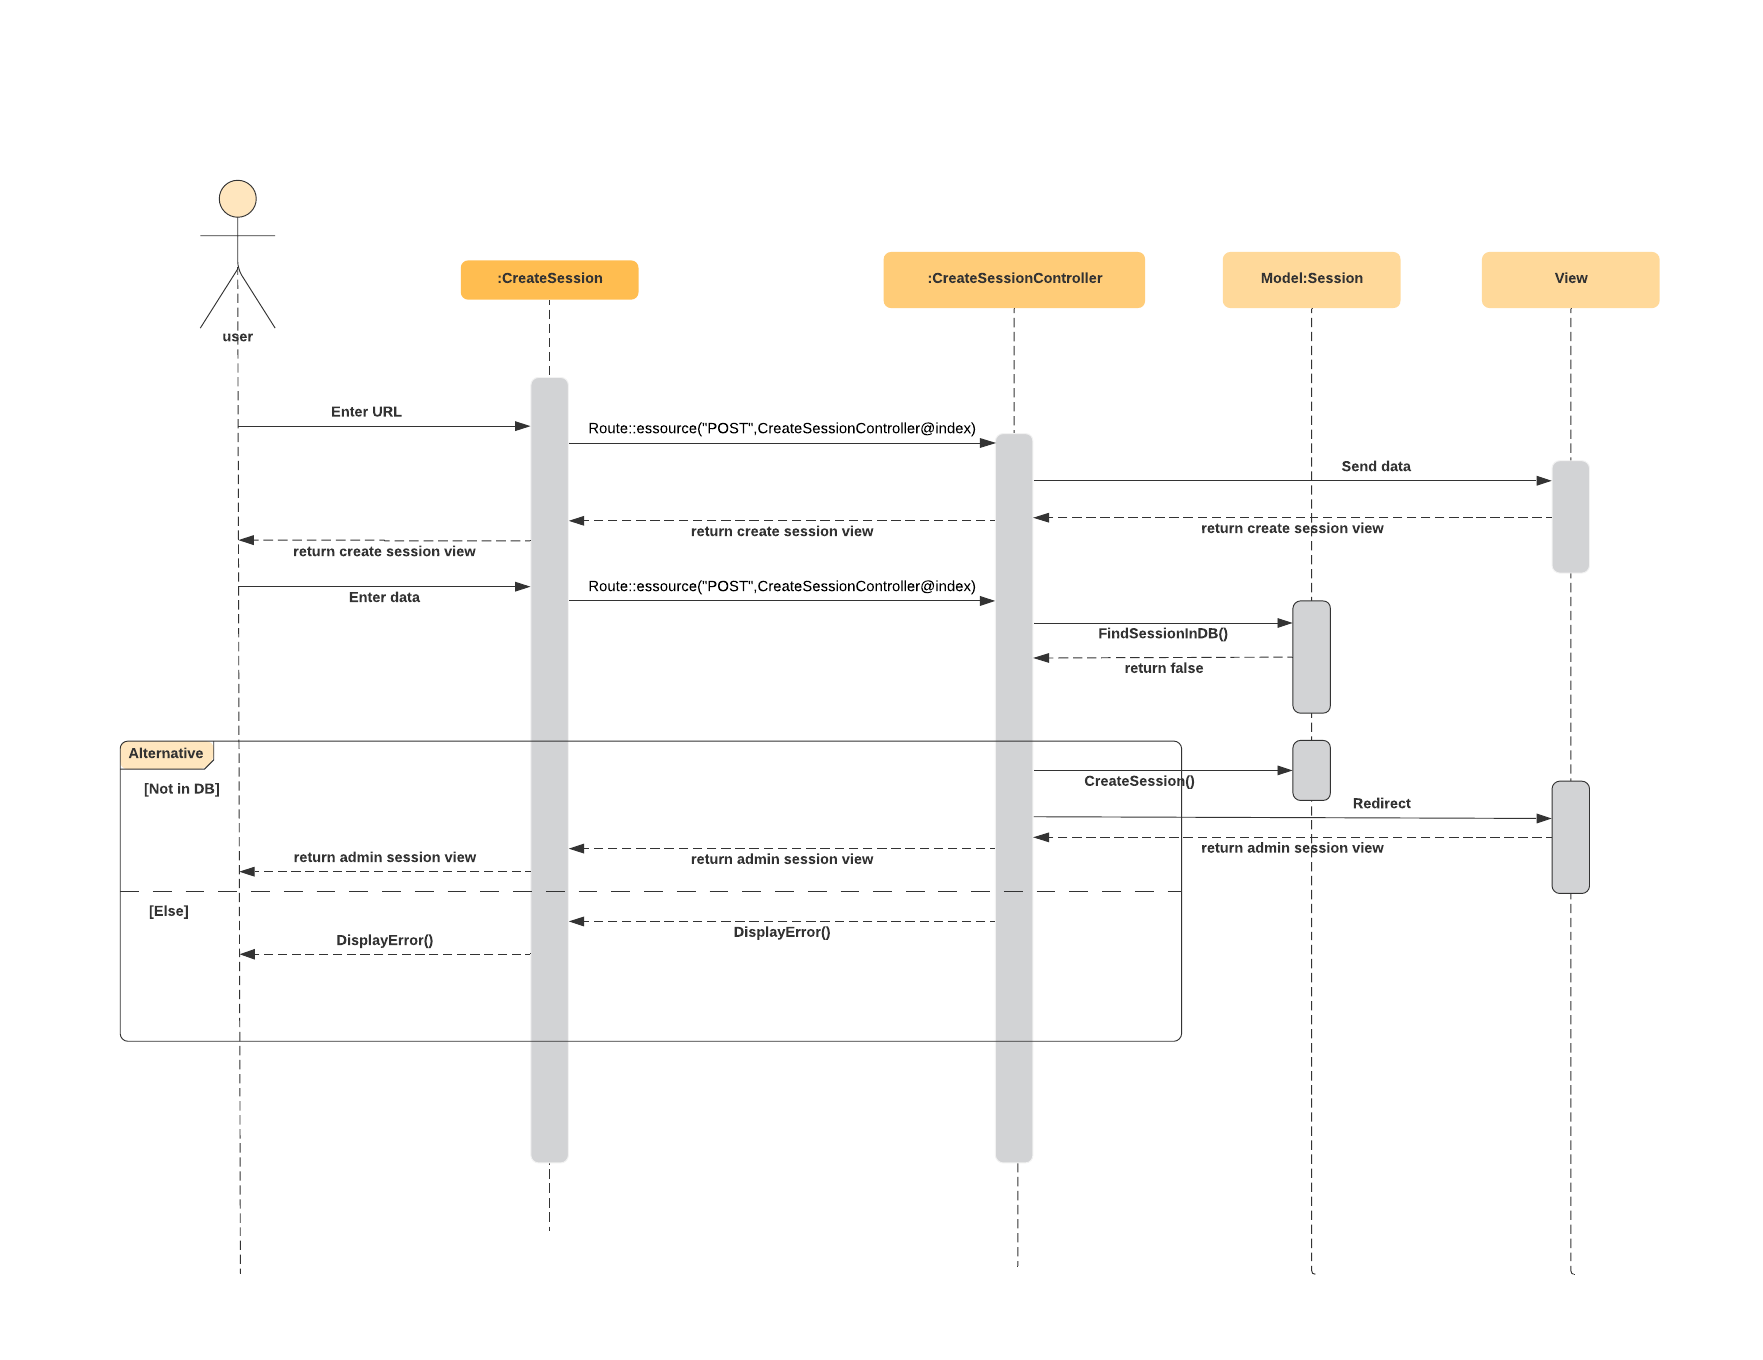
\includegraphics[width=\textwidth,center]{Diagramme/sequence-us11}
		\caption{Diagramme de séquence de l'ajout d'une session}
	\end{figure}

\vspace{\baselineskip}
\subsubsection{Scripts concerné}
	\begin{itemize}
		\item \Href{https://github.com/victorsmits/Aquabike/blob/master/Symfony-Twig/src/Entity/Session.php}{Session.php}
		\item \Href{https://github.com/victorsmits/Aquabike/blob/master/Symfony-Twig/src/Controller/CreateSessionController.php}{CreateSessionController.php}
		\item \Href{https://github.com/victorsmits/Aquabike/blob/master/Symfony-Twig/templates/create_session/session.html.twig}{session.html.twig}
	\end{itemize}